\documentclass{article}
\usepackage[utf8]{inputenc}
\usepackage{gensymb}
\usepackage{hyperref}
\hypersetup{colorlinks=true,urlcolor=blue}
\usepackage{natbib}
\usepackage{graphicx}
\usepackage{indentfirst}
\usepackage{verbatim}
\usepackage{listings}
\usepackage[verbose]{wrapfig}
\usepackage{environ}
\usepackage{lipsum}
\lstset{
basicstyle=\small\ttfamily,
columns=flexible,
breaklines=true
}
%\usepackage[tikz]{bclogo}
\usepackage{marginnote}
\usepackage{graphicx}
\usepackage{pdflscape}
%\usepackage[paper=portrait,pagesize]{typearea}
\usepackage[T1]{fontenc}

\begin{document}
\begin{titlepage}
  \begin{figure}[t]
    \centering
    
\includegraphics[]{../Figuras_Globales/00_unr.png}
    \hspace{0.15\textwidth}
    
\includegraphics[width=0.4\textwidth]{../Figuras_Globales/00_eim.png}
\end{figure}
  
\begin{center}
    {\Huge Informe N\degree2:\\ Estudio de caso axisimétrico \par}
    
    %\date{November 2019}
    
    %\bigskip\bigskip\bigskip\bigskip\bigskip\bigskip
    \begin{figure}[h]
        \centering
        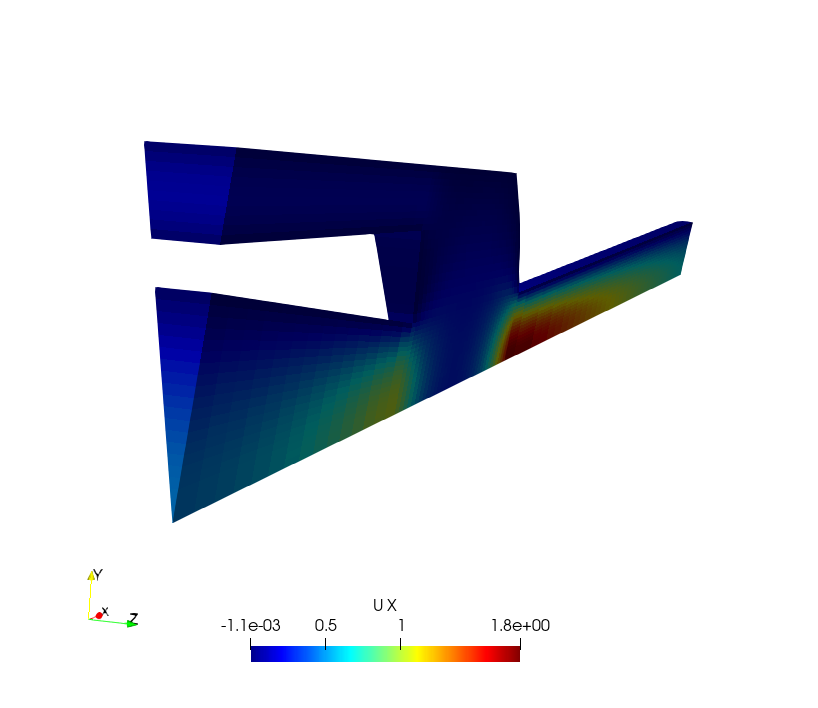
\includegraphics[width=0.7\textwidth]{Figuras/00_intro2.png}
    \end{figure}
    %\bigskip
    {\Huge Resumen:\\}
   Preparación de un caso con axisimetría utilizando la malla generada con \textit{blockMesh} en el informe anterior. Comparación de resultados utilizando ambas mallas.
    
    \bigskip
    \vspace*{\fill}
    Autor: Guillermo Rolle\par
    Supervisor: Dr. Ing. César Pairetti\par
    \bigskip
    Diciembre 2019
\end{center}
\end{titlepage}

%\maketitle
\tableofcontents
\newpage

\section{Introducción}
En este trabajo se mostrará cómo modificar una malla creada con \textit{blockMesh} para realizar un estudio de un problema axisimétrico.\par
Modificaremos la malla creada en el \href{https://github.com/guillerolle/informes_cfd/blob/master/Informe01.pdf}{Informe01} para que represente tubos de sección circular. No es necesario crear toda la geometría en 3D porque existen herramientas de OpenFOAM para aprovechar la simetría del problema. Solamente habrá 1 celda en la dirección del eje Z, pero esta vez la sección tendrá forma de "porción de pizza" para representar una sección cilíndrica.

\begin{figure}[h!]
	\centering
	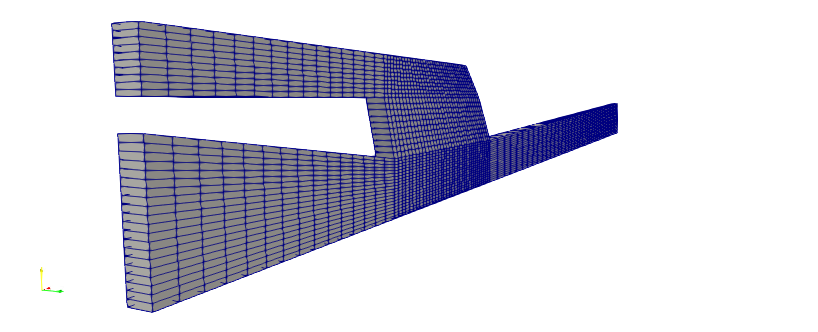
\includegraphics[width=1\textwidth]{Figuras/01_comp_01.png}
	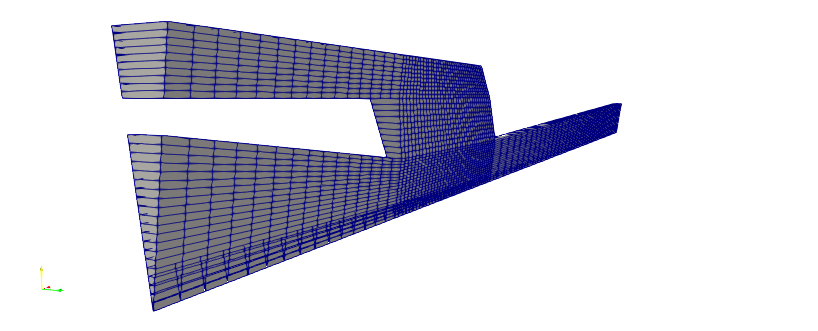
\includegraphics[width=1\textwidth]{Figuras/01_comp_02.png}
	\caption{Comparación de la geometría. Original (arriba). Modificado (abajo)}
	\label{fig:preliminar}
\end{figure}


\subsection{Información preliminar del problema}

Utilizaremos exactamente los mismos parámetros que el caso anterior para independizar mejor los cambios debido a la simetría de la malla. Las presiones a las entradas y salida son las mismas y también lo son las tolerancias de los métodos numéricos.
El caso final preparado correspondiente a este informe se encuentra en el \href{https://github.com/guillerolle/casos_cfd/tree/master/02}{repositorio}.

\section{Preparación del caso}
Comenzaremos generando una copia del \href{https://github.com/guillerolle/casos_cfd/tree/master/01}{caso 01} y eliminamos el directorio con toda la información correspondiente a la malla en \texttt{./constant/polyMesh}
\marginnote{\small \textbf{OpenFOAM tips:\\} Recordar que debe estar cargado el entorno OpenFOAM en la terminal}
\begin{lstlisting}
$ cd casos_cfd
$ mkdir 02
$ cp -r ./01 ./02
$ cd 02
$ rm -r constant/polyMesh
\end{lstlisting}

Para realizar la simetría, es necesario que las caras "frontAndBack" definidas en el diccionario \href{https://github.com/guillerolle/casos_cfd/blob/master/02/system/blockMeshDict}{blockMeshDict}  sean 2 diferentes.

Es decir, modificar esto:
\begin{lstlisting}
empty frontAndBack
(
(0 1 12 13)
(1 2 5 12)
(2 3 4 5)
(12 5 6 11)
(11 6 7 8)
(10 11 8 9)

(14 27 26 15)
(15 26 19 16)
(16 19 18 17)
(26 25 20 19)	
(25 22 21 20)
(24 23 22 25)
)
\end{lstlisting}
Por esto
\begin{lstlisting}
empty front
(
(0 1 12 13)
(1 2 5 12)
(2 3 4 5)
(12 5 6 11)
(11 6 7 8)
(10 11 8 9)
)
empty back
(
(14 27 26 15)
(15 26 19 16)
(16 19 18 17)
(26 25 20 19)
(25 22 21 20)
(24 23 22 25)
)
\end{lstlisting}
%\marginnote{\small \textbf{Linux tips:\\} '..' representa el directorio superior}

%\noindent Ver archivo completo: \href{https://github.com/guillerolle/casos_cfd/blob/master/01/constant/turbulenceProperties}{constant/turbulenceProperties}
%\lstinputlisting[caption=\textit{constant/turbulenceProperties},frame=shadowbox]{OpenFOAM/turbulenceProperties.txt}

\subsection{Mallado Inicial}
Crearemos la malla con \textit{blockMesh}. El resultado será la misma malla que el caso anterior pero si lo observamos en \textit{ParaView}, las caras "front" y "back" son ahora 2 componentes distintas.

\begin{figure}[h!]
	\centering
	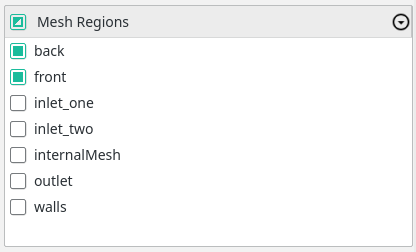
\includegraphics[width=1\textwidth]{Figuras/02_mesh_regions.png}
	\caption{Regiones de malla en ParaView}
	\label{fig:preliminar}
\end{figure}

Para crear la simetría utilizaremos la función \href{https://www.openfoam.com/documentation/guides/latest/man/extrudeMesh.html}{extrudeMesh}. Necesitamos crear un diccionario en la carpeta \textit{system} llamado \textit{extrudeMeshDict}. Podemos copiar uno de los casos tutorial de \textit{OpenFOAM} o mejor podemos descargar uno directamente del repositorio en cuestión: \href{https://github.com/guillerolle/casos_cfd/blob/master/02/system/extrudeMeshDict}{extrudeMeshDict}.\par
En este diccionario se define las caras de "cuña" (wedge), el eje de simetría y el ángulo de la extrusión.

\begin{lstlisting}
constructFrom patch;
sourceCase "$FOAM_CASE";
sourcePatches (front);

// If construct from patch: patch to use for back (can be same as sourcePatch)
exposedPatchName back;
....
//- Linear extrusion in point-normal direction
extrudeModel        wedge;

point (0 0 0);
// punto de paso del eje
axis (1 0 0);
// direccion del eje de simetria
angle 15;
// angulo de la seccion circular
....
\end{lstlisting}

Ahora podemos ejecutar la utilidad \textit{extrudeMesh}

\begin{lstlisting}
$ extrudeMesh 
\end{lstlisting}

\begin{figure}[h!]
	\centering
	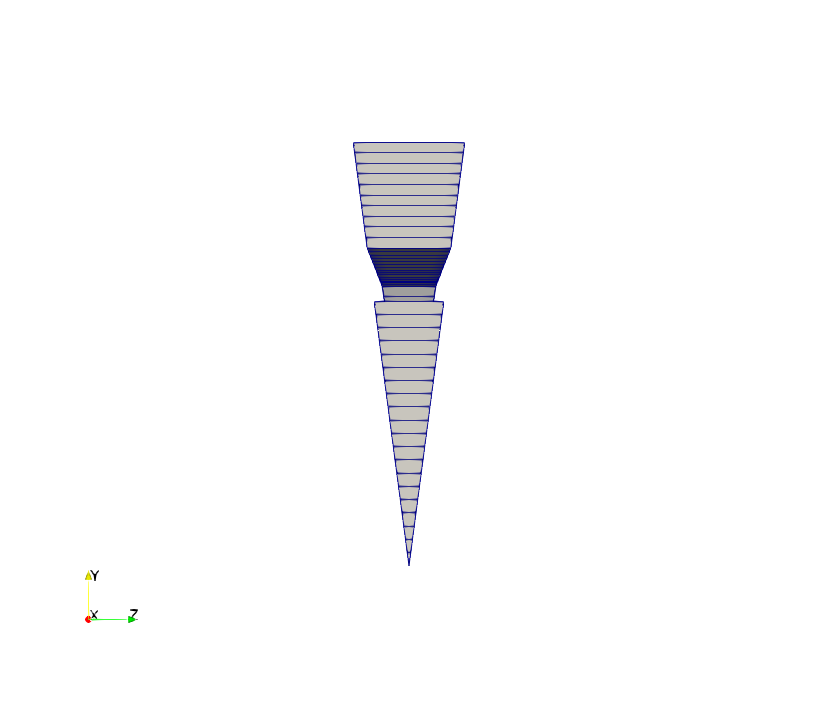
\includegraphics[width=0.4\textwidth]{Figuras/02_pizza.png}
	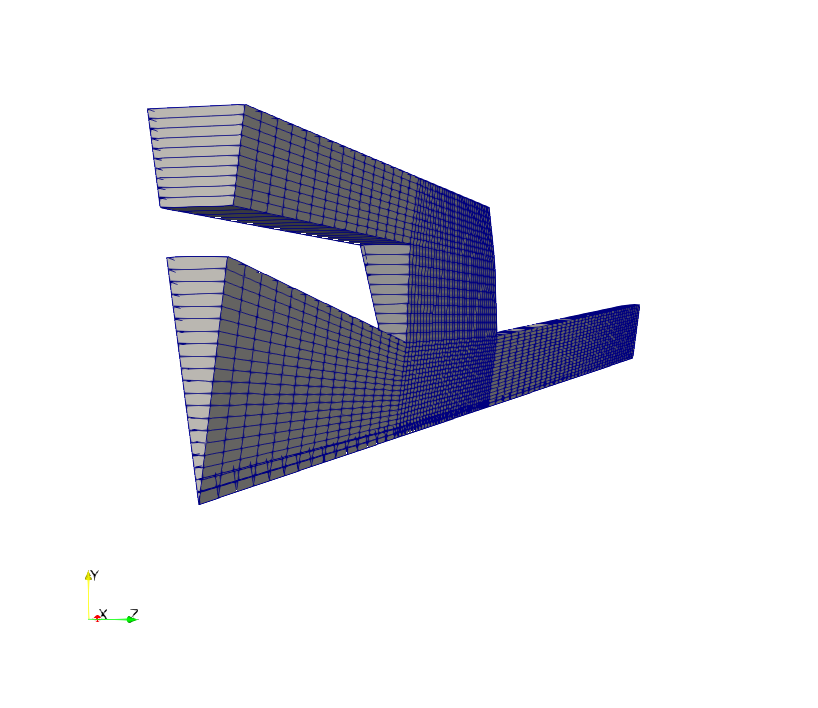
\includegraphics[width=0.4\textwidth]{Figuras/02_pizza2.png}
	\caption{Sección con forma de 'porción de pizza' en ParaView}
	\label{fig:preliminar}
\end{figure}

\marginnote{\small \textbf{Linux tips:\\} Es posible escribir un script de comandos de Linux y ejecutarlos con \texttt{./script.sh}. Ver \textit{comandos.sh}}
Sería interesante observar el resultado de \textit{checkMesh} para encontrar errores en la malla. Podemos ver que hay errores debido a que, por ejemplo, hay ciertas caras que resultaron ser "aplastadas" (las del eje central) en la extrusión en cuña. Estas caras tienen área nula, lo que es problemático a la hora de resolver las simulaciones.

\subsection{Reparacion de la malla}
Podemos utilizar la funcionalidad \href{https://openfoamwiki.net/index.php/CollapseEdges}{collapseEdges} para reparar la malla. Esta utilidad colapsa aristas pequeñas y combina aristas que estén en línea.

\begin{lstlisting}
$ collapseEdges -overwrite
\end{lstlisting}

Una vez más, comprobamos con \textit{checkMesh} para verificar que no haya inconvenientes con la malla:

\begin{lstlisting}
$ checkMesh
...
Checking geometry...
Overall domain bounding box (0 0 -0.00104421) (0.1 0.00793156 0.00104421)
Mesh has 2 geometric (non-empty/wedge) directions (1 1 0)
Mesh has 3 solution (non-empty) directions (1 1 1)
Wedge front with angle 7.50001 degrees
Wedge back with angle 7.50001 degrees
All edges aligned with or perpendicular to non-empty directions.
Boundary openness (-5.20681e-21 -2.03166e-15 2.13322e-15) OK.
Max cell openness = 2.62994e-16 OK.
Max aspect ratio = 22.9592 OK.
Minimum face area = 2.91172e-09. Maximum face area = 2.2737e-06.  Face area magnitudes OK.
Min volume = 1.24767e-12. Max volume = 5.46506e-10.  Total volume = 3.41533e-07.  Cell volumes OK.
Mesh non-orthogonality Max: 51.1811 average: 16.3359
Non-orthogonality check OK.
Face pyramids OK.
Max skewness = 0.930108 OK.
Coupled point location match (average 0) OK.

Mesh OK.

End
\end{lstlisting}

\section{Preparación de la simulación}
Vamos a utilizar las mismas condiciones iniciales y mismos diccionarios que en el otro caso. Sin embargo, debemos actualizar los archivos \texttt{0/U} y \texttt{0/p} con los parches \textit{front} y \textit{back} como las definimos anteriormente.

También, debemos modificar el tipo de los parches de \textit{empty} a \textit{wedge}. \href{https://www.openfoam.com/documentation/user-guide/boundaries.php}{Ver más información sobre boundaries}

Las modificaciones en los archivos son (en ambos):
\begin{lstlisting}
    front
{
type            wedge;
}
back
{
type            wedge;
}
}
\end{lstlisting}

\noindent Ver los archivos completos: 
\href{https://github.com/guillerolle/casos_cfd/tree/master/02/0/U}{0/U};
\href{https://github.com/guillerolle/casos_cfd/tree/master/02/0/p}{0/p}

\bigskip
Los otros diccionarios en \textit{system}, como \textit{fvSolution} y \textit{fvSchemes}, los dejamos entonces sin modificar como en la simulación anterior.

%\newpage
\section{Simulación: \textit{\href{https://openfoamwiki.net/index.php/SimpleFoam}{simpleFoam}}}
En este caso, la simulación no converge. Podemos ver que calcula hasta la última iteración definida en el \textit{controlDict}.
Volvemos a ejecutar la simulación y procesamos los archivos log para verificar los residuales. Luego los graficamos entrando a la carpeta \texttt{./logs} con \textit{gnuplot}.

\begin{lstlisting}
$ simpleFoam | tee log.simpleFoam
$ foamLog log.simpleFoam
$ gnuplot 
> load 'graficar_res.gp'
\end{lstlisting}
\marginnote{\small \textbf{gnuplot tips:\\} Es posible escribir un script de comandos de gnuplot y ejecutarlos con \texttt{gnuplot <script.gp>} o desde gnuplot con \texttt{'load <script.gp>'}}

\begin{figure}[h!]
	\centering
	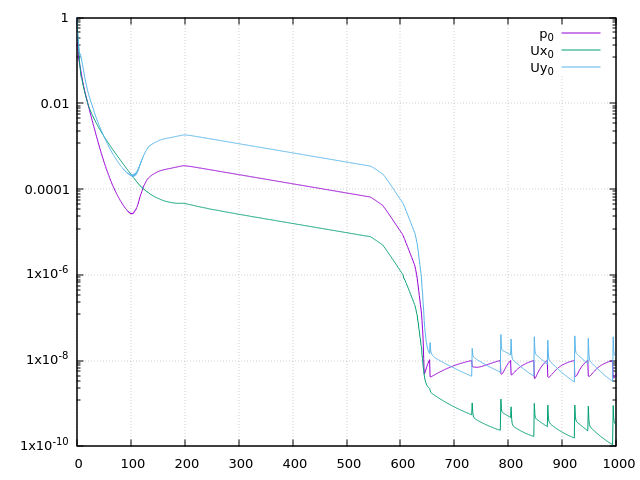
\includegraphics[width=1\textwidth]{Figuras/04_residuales_noconv.png}
	\caption{Residuales no convergentes}
	\label{fig:resid_noconv}
\end{figure}

Esto es así porque \textit{simpleFoam} está intentando resolver para Uz también por la simetría y ese valor no converge.
Para solucionarlo vamos a evitar controlar por Uz por fines prácticos. Para eso, debemos modificar en el archivo \texttt{system/fvSolution}:
\begin{lstlisting}
Esta linea: U			1e-5;
Por esta:   "(Ux|Uy)"           1e-5;
\end{lstlisting}

\noindent Ver archivo completo: \href{https://github.com/guillerolle/casos_cfd/blob/master/02/system/fvSolution}{system/fvSolution}

\newpage
Podemos ejecutar la simulación nuevamente con los mismos comandos anteriores y vemos los residuales nuevamente. Esta vez, con Uz también:

\begin{figure}[h!]
	\centering
	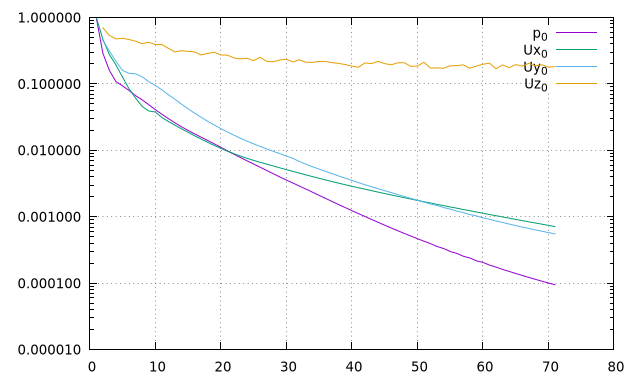
\includegraphics[width=1\textwidth]{Figuras/04_residuales_siconv.png}
	\caption{Residuales convergentes}
	\label{fig:resid_siconv}
\end{figure}

Nótese que no se controla por Uz.

\bigskip
En la figura \ref{fig:sF_Ux} se compara el perfil de velocidad (componente X) obtenido en el caso axisimétrico y en el caso previo. Se observa que el valor máximo es mayor en el caso axisimétrico y además se encuentra sobre el eje de simetría.\par 
Otra observación interesante que podemos realizar en la misma figura, es que en este nuevo caso hay una mayor cantidad de líneas de traza provenientes de la entrada de agroquímico. Esto nos permite sospechar un aumento de la concentración final en la salida, una vez hayamos terminado la simulación RTD.
\begin{figure}[h!]
	\centering
	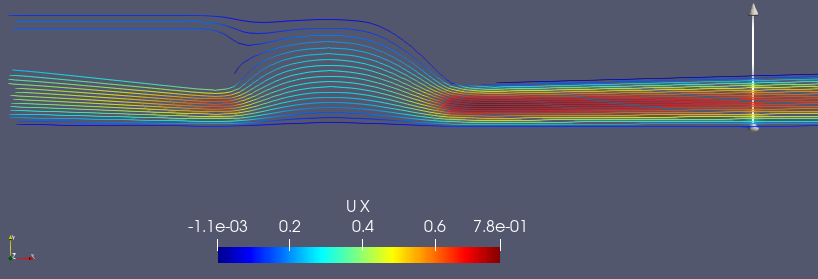
\includegraphics[width=0.85\textwidth]{../Informe01/Figuras/stream_vel.png}
	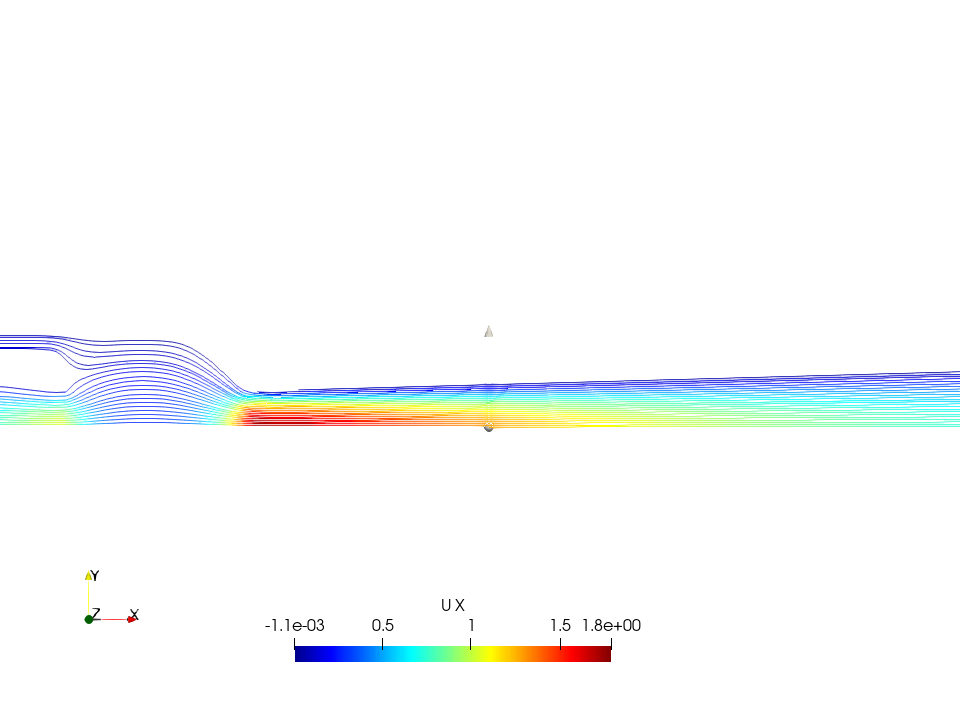
\includegraphics[width=0.85\textwidth]{Figuras/04_traza.png}
	\caption{Líneas de traza. Escala de velocidad $U_x$. Informe01 (arriba), Informe02 (abajo)}
	\label{fig:sF_Ux}
\end{figure}

\newpage
\section{Preparación del caso RTD}
Una vez obtenido el campo de velocidad con \textit{simpleFoam}, preparamos el caso RTD. Dentro del directorio del caso principal, creamos una carpeta llamada "RTD" y usaremos de plantilla el caso RTD del informe anterior.
Reemplazamos las condiciones iniciales de velocidad por el resultado final de la última simulación (en este caso, iteración número 71):
\begin{lstlisting}
$ mkdir RTD
$ cd RTD/
$ cp ../71/U ./0
\end{lstlisting}
Debemos modificar las condiciones de "T" de manera que coincidan con los patches definidos en la malla nueva. \href{https://github.com/guillerolle/casos_cfd/tree/master/02/RTD/0/T}{Ver 0/T}.\par
Copiamos la malla generada antes al nuevo caso:
\begin{lstlisting}
$ cp -r ../constant/polyMesh ./constant
\end{lstlisting}
\marginnote{\small \textbf{Linux tips:\\} El comando \texttt{cp -r} indica una copia recursiva. Es decir, permite copiar directorios completos en lugar de archivos puntuales. Ver \texttt{man cp}}

Los otros archivos en \texttt{constant} y \texttt{system} los dejamos como en el caso anterior. En el siguiente link se encuentra el directorio principal del caso RTD correspondiente a este informe: \href{https://github.com/guillerolle/casos_cfd/tree/master/02/RTD}{RTD - 02}

\section{Simulación: \textit{scalarTransportFoam}}
Ya tenemos el caso RTD preparado y podemos ejecutar la simulación con el solver \textit{scalarTransportFoam}. Cabe destacar que este es un solver transitorio a diferencia de \textit{simpleFoam} que es estacionario.

\begin{lstlisting}
$ scalarTransportFoam | tee log.scalarTransportFoam
$ foamLog log.scalarTransportFoam
\end{lstlisting}

Podemos cargar el archivo de estado de ParaView \textit{RTD.pvsm} para ver las gráficas y filtros correspondientes.

\begin{figure}[h!]
	\centering
	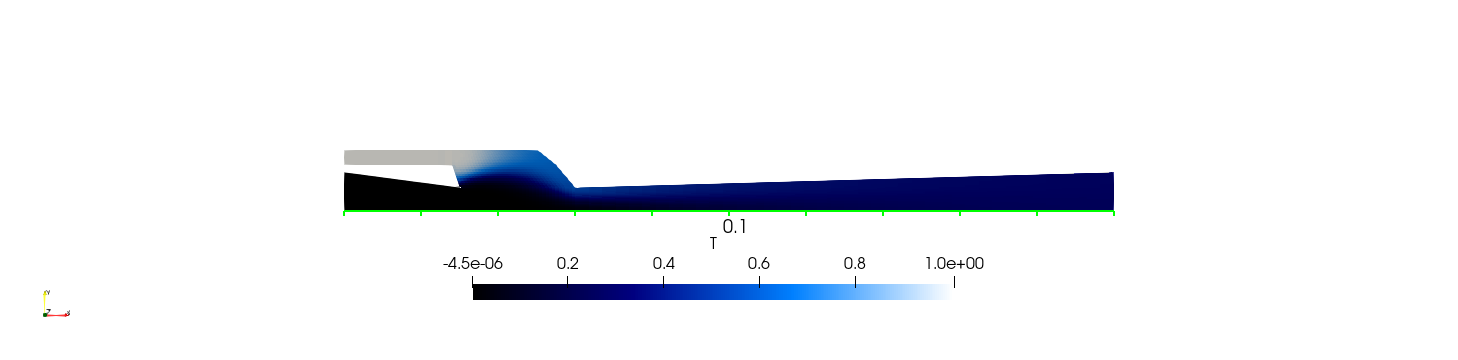
\includegraphics[width=1\textwidth]{Figuras/06_campo_T.png}
	\caption{Concentración de agroquímico (t = 2s)}
	\label{fig:campo_t}
\end{figure}

En la figura \ref{fig:comp_t} se muestra la concentración de agroquímicos de los dos casos realizados. Se aprecia claramente un aumento en la concentración final.

\begin{figure}[h!]
	\centering
	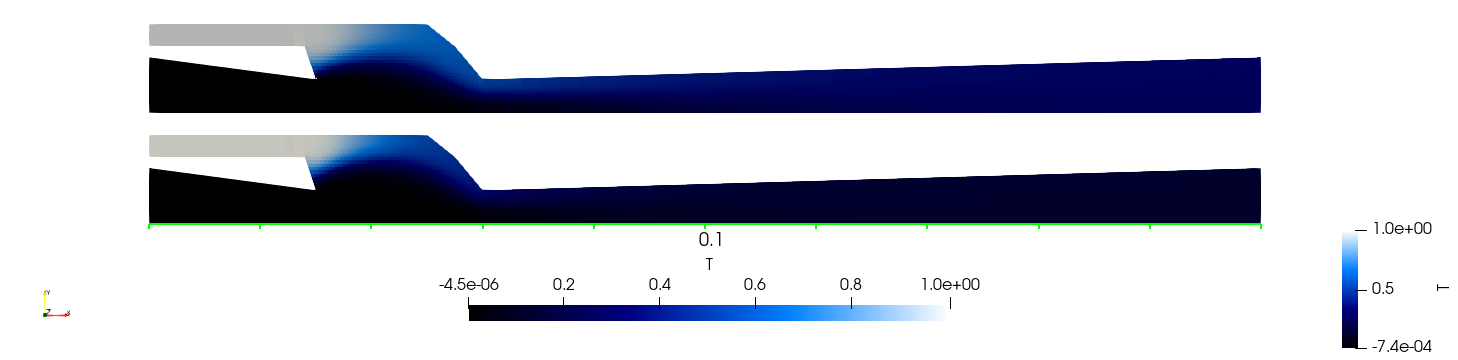
\includegraphics[width=1\textwidth]{Figuras/06_comparacion_T.png}
	\caption{Concentración - Informe01 (abajo), Informe02 (arriba)}
	\label{fig:comp_t}
\end{figure}

\newpage
\section{Post proceso}
Para obtener el valor promedio de concentración a la salida, podemos utilizar la función \textit{patchAverage} definida en el caso anterior.

\begin{lstlisting}
$ postProcess -func 'patchAverage'
\end{lstlisting}

Esto nos crea una carpeta \texttt{postProcess} con los resultados. Graficamos ahora en \textit{gnuplot}:

\begin{lstlisting}
$ gnuplot
> cd 'postProcessing/patchAverage/0'
> set term wxt 0
> plot 'surfaceFieldValue.dat' w l title "outlet"
> set xlabel "Tiempo [s]"
> set ylabel "Concentracion []"
> set grid
> replot
\end{lstlisting}

\begin{figure}[h!]
	\centering
	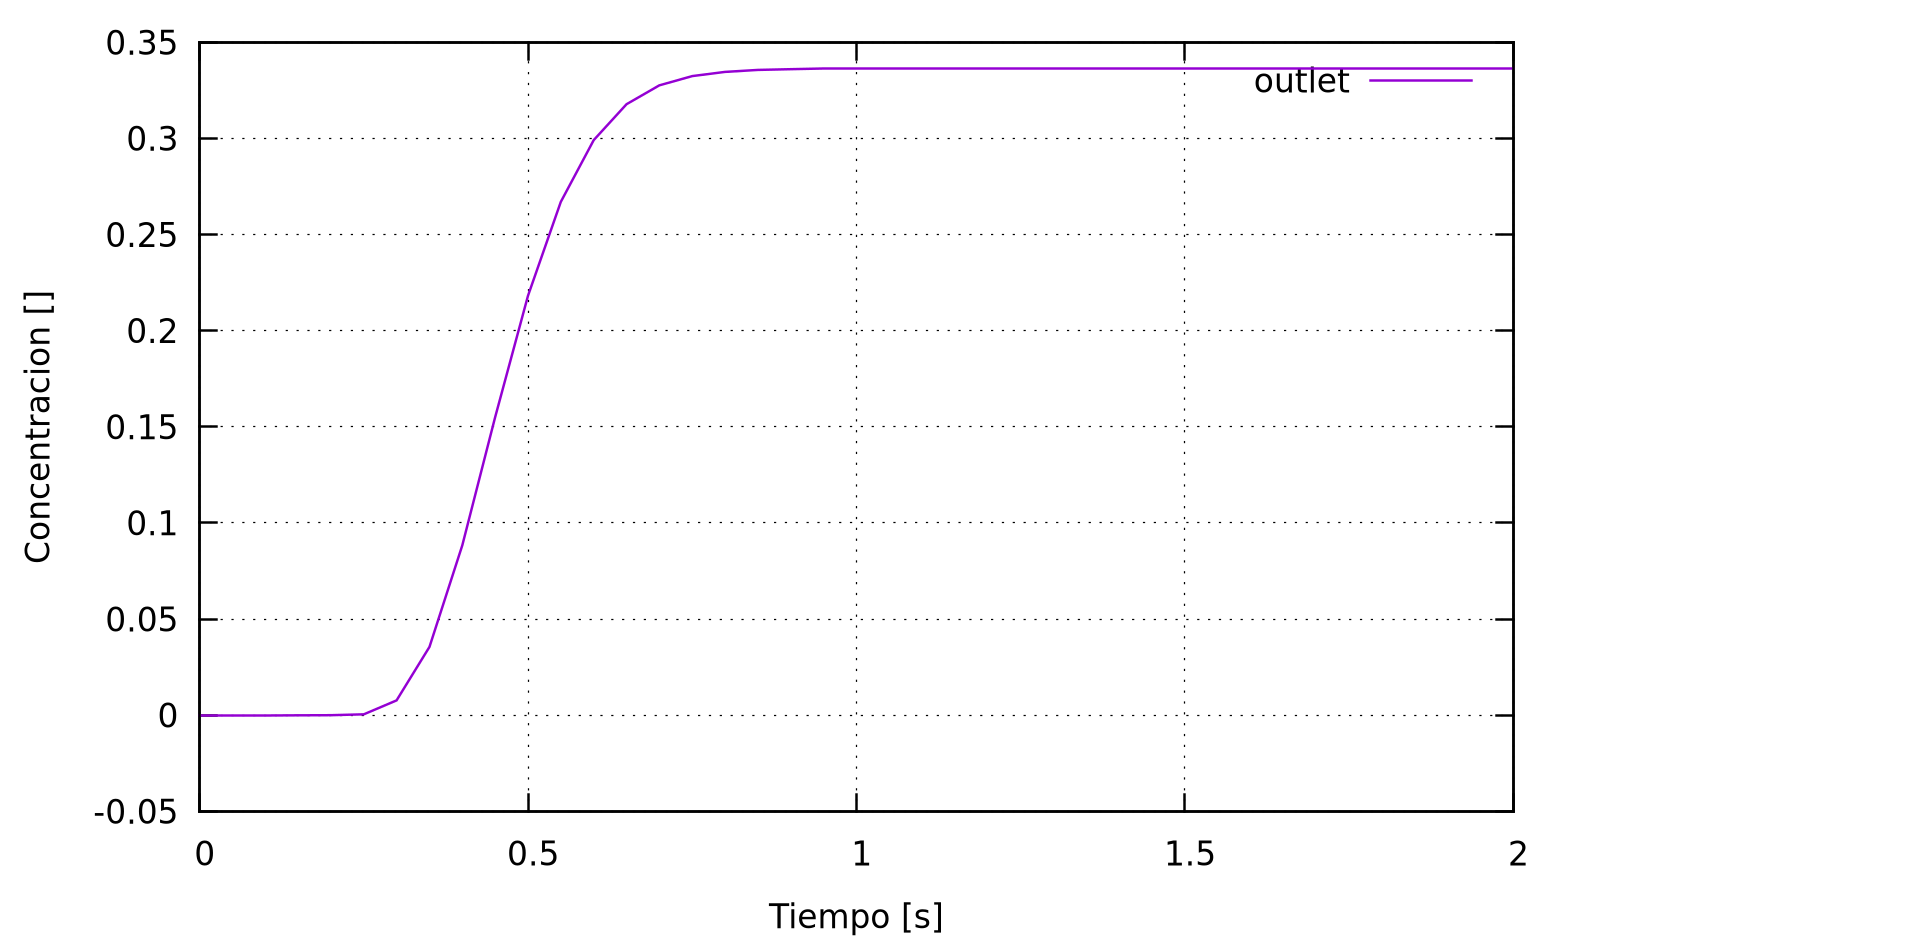
\includegraphics[width=1\textwidth]{Figuras/07_patchAverage.png}
	\caption{Concentración en la salida en función del tiempo}
	\label{fig:curva_conc}
\end{figure}

Por último, verificar el perfil de concentración y comparar el perfil de velocidad a la salida en ambos casos con ParaView.

En la figura \ref{fig:curva_conc} se observa que la concentración en la salida no es completamente uniforme. Ésta oscila en un rango del 1.5\%

\begin{figure}[h!]
	\centering
	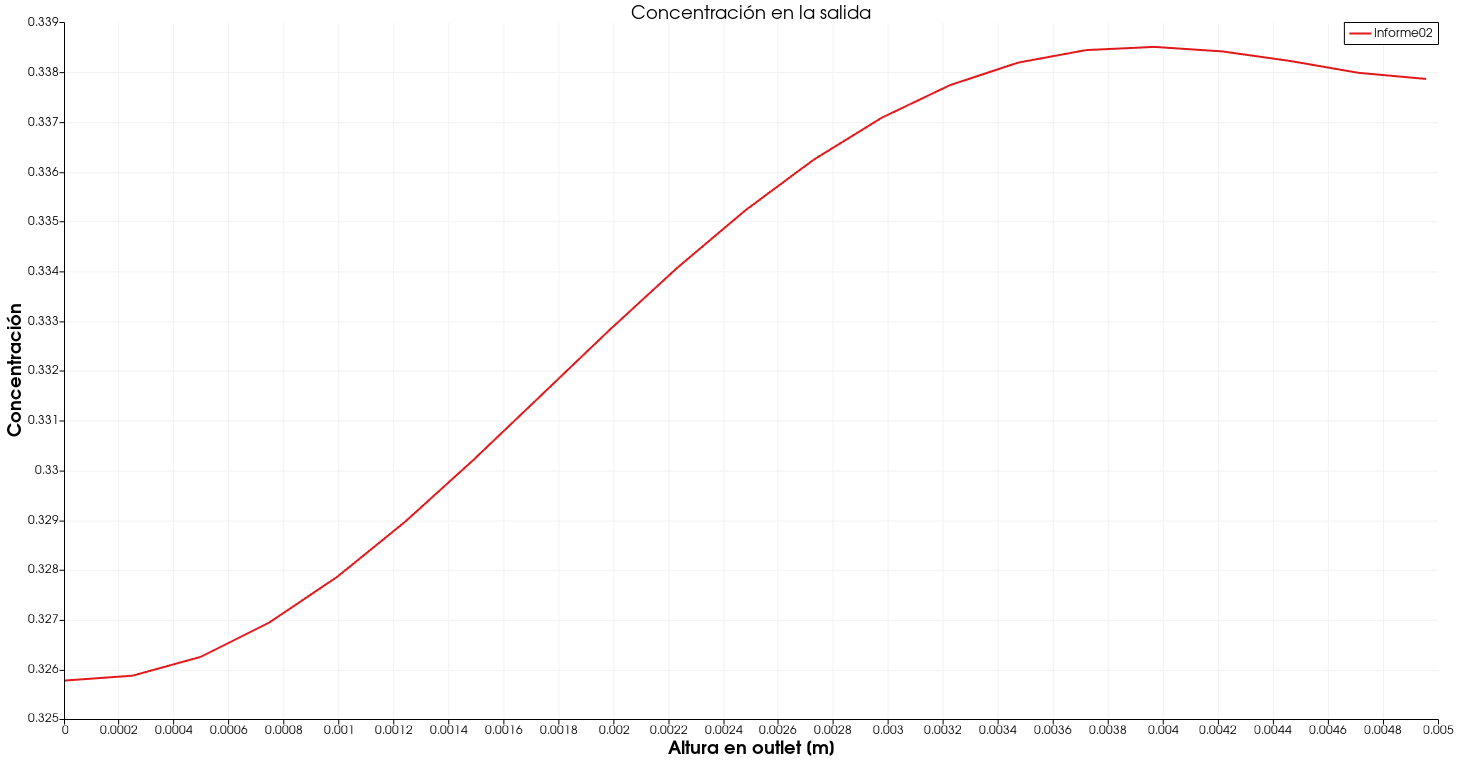
\includegraphics[width=1\textwidth]{Figuras/07_perfilT.png}
	\caption{Perfil de concentración a la salida}
	\label{fig:curva_conc}
\end{figure}

Es interesante comparar el perfil de velocidad en los dos casos. En la figura \ref{fig:curva_comp_ux} se observa que en el caso axisimétrico (Informe02) la velocidad del fluido alcanza un máximo bastante mayor al del primer caso, y, como era de esperar, ese máximo se encuentra sobre el eje central de la malla.

\begin{figure}[h!]
	\centering
	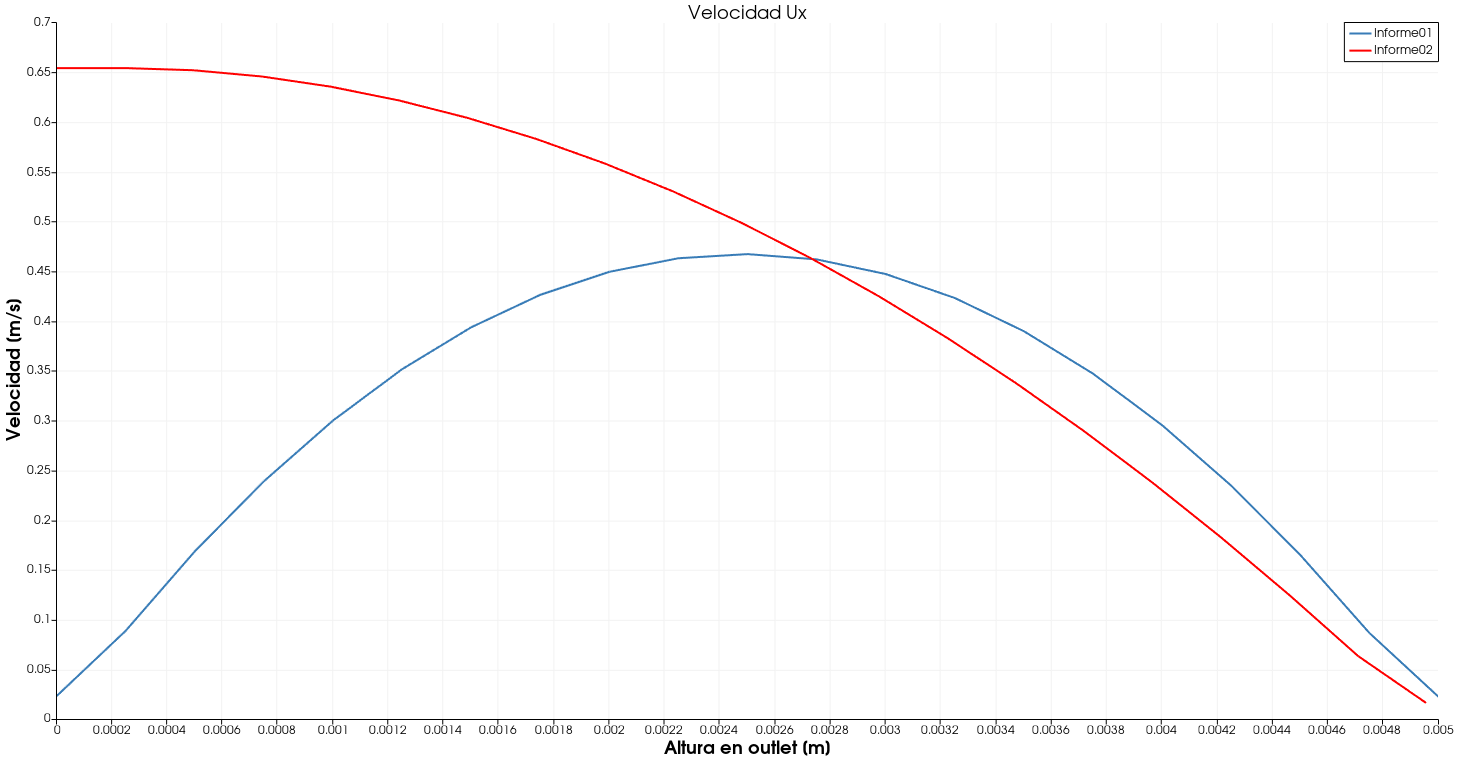
\includegraphics[width=1\textwidth]{Figuras/07_comparacion_Ux.png}
	\caption{Perfil de velocidad $U_x$ en la salida}
	\label{fig:curva_comp_ux}
\end{figure}



\end{document}
